\documentclass[]{article}
\usepackage{lmodern}
\usepackage{amssymb,amsmath}
\usepackage{ifxetex,ifluatex}
\usepackage{fixltx2e} % provides \textsubscript
\ifnum 0\ifxetex 1\fi\ifluatex 1\fi=0 % if pdftex
  \usepackage[T1]{fontenc}
  \usepackage[utf8]{inputenc}
\else % if luatex or xelatex
  \ifxetex
    \usepackage{mathspec}
  \else
    \usepackage{fontspec}
  \fi
  \defaultfontfeatures{Ligatures=TeX,Scale=MatchLowercase}
\fi
% use upquote if available, for straight quotes in verbatim environments
\IfFileExists{upquote.sty}{\usepackage{upquote}}{}
% use microtype if available
\IfFileExists{microtype.sty}{%
\usepackage{microtype}
\UseMicrotypeSet[protrusion]{basicmath} % disable protrusion for tt fonts
}{}
\usepackage[margin=1in]{geometry}
\usepackage{hyperref}
\hypersetup{unicode=true,
            pdftitle={Statistical Inference},
            pdfauthor={Himank Jain},
            pdfborder={0 0 0},
            breaklinks=true}
\urlstyle{same}  % don't use monospace font for urls
\usepackage{color}
\usepackage{fancyvrb}
\newcommand{\VerbBar}{|}
\newcommand{\VERB}{\Verb[commandchars=\\\{\}]}
\DefineVerbatimEnvironment{Highlighting}{Verbatim}{commandchars=\\\{\}}
% Add ',fontsize=\small' for more characters per line
\usepackage{framed}
\definecolor{shadecolor}{RGB}{248,248,248}
\newenvironment{Shaded}{\begin{snugshade}}{\end{snugshade}}
\newcommand{\AlertTok}[1]{\textcolor[rgb]{0.94,0.16,0.16}{#1}}
\newcommand{\AnnotationTok}[1]{\textcolor[rgb]{0.56,0.35,0.01}{\textbf{\textit{#1}}}}
\newcommand{\AttributeTok}[1]{\textcolor[rgb]{0.77,0.63,0.00}{#1}}
\newcommand{\BaseNTok}[1]{\textcolor[rgb]{0.00,0.00,0.81}{#1}}
\newcommand{\BuiltInTok}[1]{#1}
\newcommand{\CharTok}[1]{\textcolor[rgb]{0.31,0.60,0.02}{#1}}
\newcommand{\CommentTok}[1]{\textcolor[rgb]{0.56,0.35,0.01}{\textit{#1}}}
\newcommand{\CommentVarTok}[1]{\textcolor[rgb]{0.56,0.35,0.01}{\textbf{\textit{#1}}}}
\newcommand{\ConstantTok}[1]{\textcolor[rgb]{0.00,0.00,0.00}{#1}}
\newcommand{\ControlFlowTok}[1]{\textcolor[rgb]{0.13,0.29,0.53}{\textbf{#1}}}
\newcommand{\DataTypeTok}[1]{\textcolor[rgb]{0.13,0.29,0.53}{#1}}
\newcommand{\DecValTok}[1]{\textcolor[rgb]{0.00,0.00,0.81}{#1}}
\newcommand{\DocumentationTok}[1]{\textcolor[rgb]{0.56,0.35,0.01}{\textbf{\textit{#1}}}}
\newcommand{\ErrorTok}[1]{\textcolor[rgb]{0.64,0.00,0.00}{\textbf{#1}}}
\newcommand{\ExtensionTok}[1]{#1}
\newcommand{\FloatTok}[1]{\textcolor[rgb]{0.00,0.00,0.81}{#1}}
\newcommand{\FunctionTok}[1]{\textcolor[rgb]{0.00,0.00,0.00}{#1}}
\newcommand{\ImportTok}[1]{#1}
\newcommand{\InformationTok}[1]{\textcolor[rgb]{0.56,0.35,0.01}{\textbf{\textit{#1}}}}
\newcommand{\KeywordTok}[1]{\textcolor[rgb]{0.13,0.29,0.53}{\textbf{#1}}}
\newcommand{\NormalTok}[1]{#1}
\newcommand{\OperatorTok}[1]{\textcolor[rgb]{0.81,0.36,0.00}{\textbf{#1}}}
\newcommand{\OtherTok}[1]{\textcolor[rgb]{0.56,0.35,0.01}{#1}}
\newcommand{\PreprocessorTok}[1]{\textcolor[rgb]{0.56,0.35,0.01}{\textit{#1}}}
\newcommand{\RegionMarkerTok}[1]{#1}
\newcommand{\SpecialCharTok}[1]{\textcolor[rgb]{0.00,0.00,0.00}{#1}}
\newcommand{\SpecialStringTok}[1]{\textcolor[rgb]{0.31,0.60,0.02}{#1}}
\newcommand{\StringTok}[1]{\textcolor[rgb]{0.31,0.60,0.02}{#1}}
\newcommand{\VariableTok}[1]{\textcolor[rgb]{0.00,0.00,0.00}{#1}}
\newcommand{\VerbatimStringTok}[1]{\textcolor[rgb]{0.31,0.60,0.02}{#1}}
\newcommand{\WarningTok}[1]{\textcolor[rgb]{0.56,0.35,0.01}{\textbf{\textit{#1}}}}
\usepackage{longtable,booktabs}
\usepackage{graphicx,grffile}
\makeatletter
\def\maxwidth{\ifdim\Gin@nat@width>\linewidth\linewidth\else\Gin@nat@width\fi}
\def\maxheight{\ifdim\Gin@nat@height>\textheight\textheight\else\Gin@nat@height\fi}
\makeatother
% Scale images if necessary, so that they will not overflow the page
% margins by default, and it is still possible to overwrite the defaults
% using explicit options in \includegraphics[width, height, ...]{}
\setkeys{Gin}{width=\maxwidth,height=\maxheight,keepaspectratio}
\IfFileExists{parskip.sty}{%
\usepackage{parskip}
}{% else
\setlength{\parindent}{0pt}
\setlength{\parskip}{6pt plus 2pt minus 1pt}
}
\setlength{\emergencystretch}{3em}  % prevent overfull lines
\providecommand{\tightlist}{%
  \setlength{\itemsep}{0pt}\setlength{\parskip}{0pt}}
\setcounter{secnumdepth}{0}
% Redefines (sub)paragraphs to behave more like sections
\ifx\paragraph\undefined\else
\let\oldparagraph\paragraph
\renewcommand{\paragraph}[1]{\oldparagraph{#1}\mbox{}}
\fi
\ifx\subparagraph\undefined\else
\let\oldsubparagraph\subparagraph
\renewcommand{\subparagraph}[1]{\oldsubparagraph{#1}\mbox{}}
\fi

%%% Use protect on footnotes to avoid problems with footnotes in titles
\let\rmarkdownfootnote\footnote%
\def\footnote{\protect\rmarkdownfootnote}

%%% Change title format to be more compact
\usepackage{titling}

% Create subtitle command for use in maketitle
\providecommand{\subtitle}[1]{
  \posttitle{
    \begin{center}\large#1\end{center}
    }
}

\setlength{\droptitle}{-2em}

  \title{Statistical Inference}
    \pretitle{\vspace{\droptitle}\centering\huge}
  \posttitle{\par}
    \author{Himank Jain}
    \preauthor{\centering\large\emph}
  \postauthor{\par}
      \predate{\centering\large\emph}
  \postdate{\par}
    \date{08/08/2019}


\begin{document}
\maketitle

\hypertarget{probability}{%
\section{Probability:}\label{probability}}

Probability is a measure quantifying the likelihood that events will
occur. Probability quantifies as a number between 0 and 1, where,
sparsly speaking, 0 indicates impossibility and 1 indicates certainty.
The higher the probability of an event, the more likely it is that the
event will occur. A simple example is the tossing of a fair (unbiased)
coin. Since the coin is fair, the two outcomes (``heads'' and ``tails'')
are both equally probable; the probability of ``heads'' equals the
probability of ``tails''; and since no other outcomes are possible, the
probability of either ``heads'' or ``tails'' is 1/2 (which could also be
written as 0.5 or 50\%)

Let A and B be two events then:

\[P(A \cup B)=P(A)+P(B)-P(A \cap B) \]

if A and B are independent events then:

\(P(A\cap B)=P(A)P(B)\)

\hypertarget{probability-mass-function}{%
\subsection{Probability Mass
Function:}\label{probability-mass-function}}

\hypertarget{random-variable}{%
\subsubsection{Random variable:}\label{random-variable}}

A random variable is a numerical outcome of an experiment. Discrete or
Continuous Example : Flip of a coin (0 or 1), roll of a dice

A probability mass function evaluated at a value corresponds to the
probability that a random variable takes that value.A valid pmf must
satisfy: 1) \(P >=0\) 2) \(\sum p=1\)

Example: Consider rolling a fair (unbiased) dice. The probability of any
face turning up is \(1/6\). 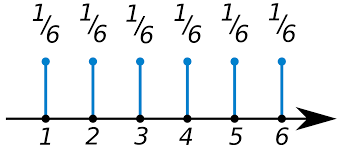
\includegraphics{pmf.png}

\hypertarget{probability-density-function}{%
\subsection{Probability Density
Function:}\label{probability-density-function}}

A probability density function (pdf) is a function associated with a
continuous random variable. A valid pdf must satisfy: 1) \[p(x)>=0\]
everywhere 2) \[ \int p(x)dx=1 \] Total area under the curve is equal to
\(1\). Area under pdf correspond to probability for that random
variable. 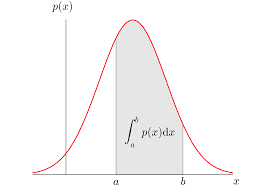
\includegraphics{pdf.png}

\hypertarget{cumulative-distribution-function-survival-function}{%
\subsubsection{Cumulative Distribution Function \& Survival
Function:}\label{cumulative-distribution-function-survival-function}}

Cumulative Distribution Function (CDF) of a random variable \(X\),
returns the probability that the random variable is less than or equal
to the value \(x\) \(F(x)=P(X<=x)\)

Survivial function of a random variable \(X\), returns the probability
that the random variable is more than the value \(x\) \(F(x)=P(X>x)\)

\hypertarget{quantiles-quartiles}{%
\subsubsection{Quantiles \& Quartiles:}\label{quantiles-quartiles}}

In statistics and probability quantiles are cut points dividing the
range of a probability distribution into continuous intervals with equal
probabilities, or dividing the observations in a sample in the same way.
There is one fewer quantile than the number of groups created. Thus
quartiles are the three cut points that will divide a dataset into four
equal-sized groups. A quartile is a type of quantile. The first quartile
(Q1) is defined as the middle number between the smallest number and the
median of the data set. The second quartile (Q2) is the median of the
data. The third quartile (Q3) is the middle value between the median and
the highest value of the data set.

\begin{figure}
\centering
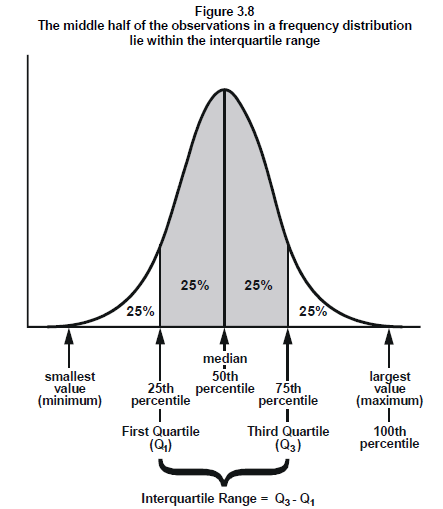
\includegraphics{quartiles.png}
\caption{quartiles}
\end{figure}

\hypertarget{conditional-probability}{%
\section{Conditional Probability:}\label{conditional-probability}}

The probability of an event A, given that another B has already
occurred. \(P(A/B)=\frac {P(A\cap B)}{P(B)}\) If A and B are
independent: \(P(A/B)=P(A)\)

\hypertarget{bayes-theorem}{%
\subsection{Bayes Theorem:}\label{bayes-theorem}}

Bayes' theorem describes the probability of an event, based on prior
knowledge of conditions that might be related to the event. For example,
if cancer is related to age, then, using Bayes theorem, a person's age
can be used to more accurately assess the probability that they have
cancer, compared to the assessment of the probability of cancer made
without knowledge of the person's age.

\(P(B/A)=\frac {P(A/B)P(B)}{P(A/B)P(B)+P(A/B')P(B')}\)

For instance, let \(+\) and \(-\) be the events that the result of a
diagnostic test is Positive or Negative respectively. Let D and D' be
the events that the subject has or does not have the disease
respectively. Then, Sensitivity = \(P(+/D)\) = \(\frac {TP}{TP+FN}\)
Specificity = \(P(-/D')\) = \(\frac {TN}{TN+FP}\) Positive Predicted
Value = \(P(D/+)\) Negative Predicted Value = \(P(D'/-)\)

\hypertarget{likelihood-ratio}{%
\subsubsection{Likelihood ratio:}\label{likelihood-ratio}}

Likelihood ratios are used for assessing the value of performing a
diagnostic test. They use the sensitivity and specificity of the test to
determine whether a test result usefully changes the probability that a
condition exists. \(\frac{P(D/+)}{P(D'/+)}\)=\(\frac{P(+/D)}{P(+/D')}\)
x \(\frac{P(D)}{P(D')}\) i.e.~ Post-test-odds= DLR+ x Pre-test-odds DLR+
= \(\frac {Sensitivity}{1-Specificity}\) This means if DLR+ is 50 then,
given the test is positive the probability of disease increases by 50
times than before the test. Similarly, DLR- =
\(\frac {1-Sensitivity}{Specificity}\) This means if DLR- is 0.003 then,
given the test is negative the probability of disease changes by 0.003
times than before the test.

\hypertarget{expected-values}{%
\subsection{Expected Values:}\label{expected-values}}

In probability theory, the expected value of a random variable is the
long-run average value of repetitions of the same experiment it
represents. For example, the expected value in rolling a six-sided die
is 3.5, because the average of all the numbers that come up is 3.5 as
the number of rolls approaches infinity. The \textbf{expected value} or
\textbf{mean} of a random variable is the center of its distribution

For discrete random variable \(X\) with PMF \(p(x)\), it is defined as
follows \[
E[X] = \sum_x xp(x).
\] \(E[X]\) represents the center of mass of a collection of locations
and weights, \(\{x, p(x)\}\)

\begin{figure}
\centering
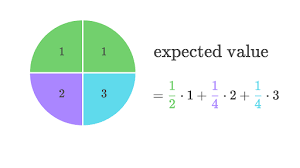
\includegraphics{expected.png}
\caption{expected value}
\end{figure}

Suppose a coin is flipped and \(X\) is declared \(0\) or \(1\)
corresponding to a head or a tail, respectively What is the expected
value of \(X\)? \[
E[X] = .5 \times 0 + .5 \times 1 = .5
\]

\begin{center}\includegraphics{stat-inf_files/figure-latex/unnamed-chunk-1-1} \end{center}

Suppose that a die is rolled and \(X\) is the number face up What is the
expected value of \(X\)? \[
E[X] = 1 \times \frac{1}{6} + 2 \times \frac{1}{6} +
3 \times \frac{1}{6} + 4 \times \frac{1}{6} +
5 \times \frac{1}{6} + 6 \times \frac{1}{6} = 3.5
\]

\hypertarget{continous-random-vairalbe-expected-values}{%
\subsubsection{Continous random vairalbe expected
values:}\label{continous-random-vairalbe-expected-values}}

For a continuous random variable, \(X\), with density, \(f\), the
expected value is defined as follows \[
E[X] = \mbox{the area under the function}~~~ t f(t)
\]

Consider a density where \(f(x) = 1\) for \(x\) between zero and one
Suppose that \(X\) follows this density; what is its expected value?\\
\textbf{0.5}
\includegraphics{stat-inf_files/figure-latex/unnamed-chunk-2-1.pdf}

\hypertarget{variance}{%
\section{Variance:}\label{variance}}

The variance of a random variable is a measure of its spread. If \(X\)
is a random variable with mean \(\mu\), the variance of \(X\) is defined
as

\[Var(X) = E[(X - \mu)^2]\]

the expected (squared) distance from the mean

\[Var(X) = E[X^2] - E[X]^2\]

The square root of the variance is called the \textbf{standard
deviation}.

What's the sample variance from the result of a toss of a die?

\$ E{[}X{]} = 3.5 \$ \[
E[X^2] = 1 ^ 2 \times \frac{1}{6} + 2 ^ 2 \times \frac{1}{6} + 3 ^ 2 \times \frac{1}{6} + 4 ^ 2 \times \frac{1}{6} + 5 ^ 2 \times \frac{1}{6} + 6 ^ 2 \times \frac{1}{6} = 15.17
\]

\(Var(X) = E[X^2] - E[X]^2 \approx 2.92\)

What's the sample variance from the result of the toss of a coin with
probability of heads (1) of \(p\)?
\(E[X] = 0 \times (1 - p) + 1 \times p = p\) \(E[X^2] = E[X] = p\)
\(Var(X) = E[X^2] - E[X]^2 = p - p^2 = p(1 - p)\)

\hypertarget{standard-error}{%
\subsection{Standard Error:}\label{standard-error}}

The standard error (SE) of a statistic (usually an estimate of a
parameter) is the standard deviation of its sampling distribution{[}1{]}
or an estimate of that standard deviation. If the parameter or the
statistic is the mean, it is called the standard error of the mean
(SEM). The variance of sample mean is \(\frac{\sigma^2}{n}\). Its
logical estimate is \(\frac{s^2}{n}\) The standard error of the mean:
\(\frac{s}{\sqrt{n}}\) Here, S,the standard deviation, talks about how
variable the population is \(\frac{S}{\sqrt{n}}\) talks about how
variable the averages of random samples of size n from population are.

\hypertarget{common-distributions}{%
\section{Common Distributions:}\label{common-distributions}}

A probability distribution is a mathematical function that provides the
probabilities of occurrence of different possible outcomes in an
experiment.

\hypertarget{binomial-distribution}{%
\subsection{Binomial Distribution:}\label{binomial-distribution}}

The \textbf{Bernoulli distribution} arises as the result of a binary
outcome

\begin{itemize}
\item
  Bernoulli random variables take only the values 1 and 0 with
  probabilities of \(p\) and \(1-p\) respectively
\item
  The PMF for a Bernoulli random variable \(X\) is
  \[P(X = x) =  p^x (1 - p)^{1 - x}\]
\item
  The mean of a Bernoulli random variable is \(p\) and the variance is
  \(p(1 - p)\)
\item
  If we let \(X\) be a Bernoulli random variable, it is typical to call
  \(X=1\) as a ``success'' and \(X=0\) as a ``failure''
\end{itemize}

The \emph{binomial random variables} are obtained as the sum of iid
Bernoulli trials

\begin{itemize}
\item
  In specific, let \(X_1,\ldots,X_n\) be iid Bernoulli\((p)\); then
  \(X = \sum_{i=1}^n X_i\) is a binomial random variable
\item
  The binomial mass function is
\end{itemize}

\[P(X = x) = \left(\begin{array}{c}n \\ x\end{array}\right)p^x(1 - p)^{n-x}\]

for \(x=0,\ldots,n\)

\begin{itemize}
\item
  Suppose a friend has \(8\) children (oh my!), \(7\) of which are girls
  and none are twins
\item
  If each gender has an independent \(50\)\% probability for each birth,
  what's the probability of getting \(7\) or more girls out of \(8\)
  births?
\end{itemize}

\[\left(\begin{array}{c}8 \\ 7\end{array}\right) .5^{7}(1-.5)^{1}+\left(\begin{array}{c}8 \\ 8\end{array}\right) .5^{8}(1-.5)^{0} \approx 0.04\]

\begin{Shaded}
\begin{Highlighting}[]
\KeywordTok{choose}\NormalTok{(}\DecValTok{8}\NormalTok{, }\DecValTok{7}\NormalTok{) }\OperatorTok{*}\StringTok{ }\FloatTok{.5} \OperatorTok{^}\StringTok{ }\DecValTok{8} \OperatorTok{+}\StringTok{ }\KeywordTok{choose}\NormalTok{(}\DecValTok{8}\NormalTok{, }\DecValTok{8}\NormalTok{) }\OperatorTok{*}\StringTok{ }\FloatTok{.5} \OperatorTok{^}\StringTok{ }\DecValTok{8} 
\end{Highlighting}
\end{Shaded}

\begin{verbatim}
## [1] 0.03515625
\end{verbatim}

\begin{Shaded}
\begin{Highlighting}[]
\KeywordTok{pbinom}\NormalTok{(}\DecValTok{6}\NormalTok{, }\DataTypeTok{size =} \DecValTok{8}\NormalTok{, }\DataTypeTok{prob =} \FloatTok{.5}\NormalTok{, }\DataTypeTok{lower.tail =} \OtherTok{FALSE}\NormalTok{)}
\end{Highlighting}
\end{Shaded}

\begin{verbatim}
## [1] 0.03515625
\end{verbatim}

\hypertarget{the-normal-distribution}{%
\subsection{The normal distribution}\label{the-normal-distribution}}

\begin{itemize}
\item
  A random variable is said to follow a \textbf{normal} or
  \textbf{Gaussian} distribution with mean \(\mu\) and variance
  \(\sigma^2\) if the associated density is
  \[(2\pi \sigma^2)^{-1/2}e^{-(x - \mu)^2/2\sigma^2}\]

  If \(X\) a RV with this density then \(E[X] = \mu\) and
  \(Var(X) = \sigma^2\)
\item
  We write \(X\sim \mbox{N}(\mu, \sigma^2)\)
\item
  When \(\mu = 0\) and \(\sigma = 1\) the resulting distribution is
  called \textbf{the standard normal distribution}
\item
  The standard normal density function is labeled \(\phi\)
\item
  Standard normal RVs are often labeled \(Z\)
\end{itemize}

\begin{center}\rule{0.5\linewidth}{\linethickness}\end{center}

\begin{Shaded}
\begin{Highlighting}[]
\NormalTok{zvals <-}\StringTok{ }\KeywordTok{seq}\NormalTok{(}\OperatorTok{-}\DecValTok{3}\NormalTok{, }\DecValTok{3}\NormalTok{, }\DataTypeTok{length =} \DecValTok{1000}\NormalTok{)}

\KeywordTok{plot}\NormalTok{(zvals, }\KeywordTok{dnorm}\NormalTok{(zvals), }

     \DataTypeTok{type =} \StringTok{"l"}\NormalTok{, }\DataTypeTok{lwd =} \DecValTok{3}\NormalTok{, }\DataTypeTok{frame =} \OtherTok{FALSE}\NormalTok{, }\DataTypeTok{xlab =} \StringTok{"z"}\NormalTok{, }\DataTypeTok{ylab =} \StringTok{"Density"}\NormalTok{)}

\KeywordTok{sapply}\NormalTok{(}\OperatorTok{-}\DecValTok{3} \OperatorTok{:}\StringTok{ }\DecValTok{3}\NormalTok{, }\ControlFlowTok{function}\NormalTok{(k) }\KeywordTok{abline}\NormalTok{(}\DataTypeTok{v =}\NormalTok{ k))}
\end{Highlighting}
\end{Shaded}

\includegraphics{stat-inf_files/figure-latex/unnamed-chunk-4-1.pdf}

\hypertarget{facts-about-the-normal-density}{%
\paragraph{Facts about the normal
density}\label{facts-about-the-normal-density}}

\begin{itemize}
\item
  If \(X \sim \mbox{N}(\mu,\sigma^2)\) the \(Z = \frac{X -\mu}{\sigma}\)
  is standard normal
\item
  If \(Z\) is standard normal
  \[X = \mu + \sigma Z \sim \mbox{N}(\mu, \sigma^2)\]
\item
  The non-standard normal density is
  \[\phi\{(x - \mu) / \sigma\}/\sigma\]
\end{itemize}

\begin{enumerate}
\def\labelenumi{\arabic{enumi}.}
\item
  Approximately \(68\%\), \(95\%\) and \(99\%\) of the normal density
  lies within \(1\), \(2\) and \(3\) standard deviations from the mean,
  respectively
\item
  \(-1.28\), \(-1.645\), \(-1.96\) and \(-2.33\) are the \(10^{th}\),
  \(5^{th}\), \(2.5^{th}\) and \(1^{st}\) percentiles of the standard
  normal distribution respectively
\item
  By symmetry, \(1.28\), \(1.645\), \(1.96\) and \(2.33\) are the
  \(90^{th}\), \(95^{th}\), \(97.5^{th}\) and \(99^{th}\) percentiles of
  the standard normal distribution respectively
\end{enumerate}

\begin{center}\rule{0.5\linewidth}{\linethickness}\end{center}

\hypertarget{the-poisson-distribution}{%
\subsection{The Poisson distribution}\label{the-poisson-distribution}}

\begin{itemize}
\item
  Used to model counts
\item
  The Poisson mass function is
\end{itemize}

\[P(X = x; \lambda) = \frac{\lambda^x e^{-\lambda}}{x!}\]

for \(x=0,1,\ldots\)

\begin{itemize}
\item
  The mean of this distribution is \(\lambda\)
\item
  The variance of this distribution is \(\lambda\)
\item
  Notice that \(x\) ranges from \(0\) to \(\infty\)
\end{itemize}

\begin{center}\rule{0.5\linewidth}{\linethickness}\end{center}

\hypertarget{some-uses-for-the-poisson-distribution}{%
\subsection{Some uses for the Poisson
distribution}\label{some-uses-for-the-poisson-distribution}}

\begin{itemize}
\item
  Modeling event/time data
\item
  Modeling radioactive decay
\item
  Modeling survival data
\item
  Modeling unbounded count data
\item
  Modeling contingency tables
\item
  Approximating binomials when \(n\) is large and \(p\) is small
\end{itemize}

\begin{figure}
\centering
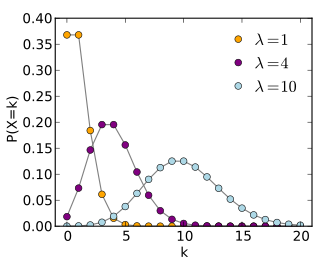
\includegraphics{pois.png}
\caption{POIS}
\end{figure}

Poisson random variables are used to model rates

\(X \sim Poisson(\lambda t)\) where \(\lambda = E[X / t]\) is the
expected count per unit of time \(t\) is the total monitoring time

\hypertarget{central-limit-theorm-law-of-large-numbers}{%
\subsection{Central Limit Theorm \& Law of Large
Numbers:}\label{central-limit-theorm-law-of-large-numbers}}

In probability theory, the central limit theorem (CLT) establishes that,
in some situations, when independent random variables are added, their
properly normalized sum tends toward a normal distribution (a ``bell
curve'') even if the original variables themselves are not normally
distributed. 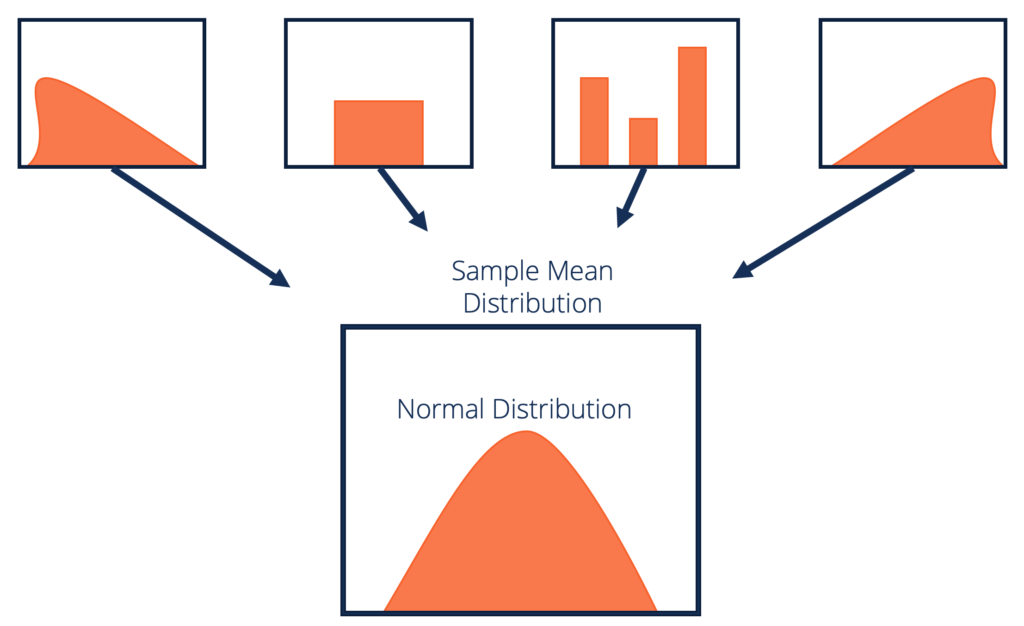
\includegraphics{CLt.png}

The law of large numbers (LLN) is a theorem that describes the result of
performing the same experiment a large number of times. According to the
law, the average of the results obtained from a large number of trials
should be close to the expected value, and will tend to become closer as
more trials are performed.

\begin{Shaded}
\begin{Highlighting}[]
\NormalTok{n <-}\StringTok{ }\DecValTok{10000}\NormalTok{; means <-}\StringTok{ }\KeywordTok{cumsum}\NormalTok{(}\KeywordTok{rnorm}\NormalTok{(n)) }\OperatorTok{/}\StringTok{ }\NormalTok{(}\DecValTok{1}  \OperatorTok{:}\StringTok{ }\NormalTok{n)}
\KeywordTok{plot}\NormalTok{(}\DecValTok{1} \OperatorTok{:}\StringTok{ }\NormalTok{n, means, }\DataTypeTok{type =} \StringTok{"l"}\NormalTok{, }\DataTypeTok{lwd =} \DecValTok{2}\NormalTok{, }\DataTypeTok{frame =} \OtherTok{FALSE}\NormalTok{, }\DataTypeTok{ylab =} \StringTok{"cumulative means"}\NormalTok{, }\DataTypeTok{xlab =} \StringTok{"sample size"}\NormalTok{)}
\KeywordTok{abline}\NormalTok{(}\DataTypeTok{h =} \DecValTok{0}\NormalTok{)}
\end{Highlighting}
\end{Shaded}

\includegraphics{stat-inf_files/figure-latex/unnamed-chunk-5-1.pdf}

\hypertarget{confidence-intervals}{%
\section{Confidence Intervals:}\label{confidence-intervals}}

In statistics, a confidence interval (CI) is a type of interval
estimate, computed from the statistics of the observed data, that might
contain the true value of an unknown population parameter.

\begin{itemize}
\item
  Therefore, according to the CLT, the probability that the random
  interval \[\bar X_n \pm z_{1-\alpha/2}\times\sigma / \sqrt{n}\]
  contains \(\mu\) is approximately 100\((1-\alpha)\)\%, where
  \(z_{1-\alpha/2}\) is the \(1-\alpha/2\) quantile of the standard
  normal distribution
\item
  This is called a \(100(1 - \alpha)\)\% \textbf{confidence interval}
  for \(\mu\)
\item
  We can replace the unknown \(\sigma\) with \(s\)
\end{itemize}

\hypertarget{poisson-interval}{%
\subsection{Poisson interval}\label{poisson-interval}}

\begin{itemize}
\item
  A nuclear pump failed 5 times out of 94.32 days, give a 95\%
  confidence interval for the failure rate per day?
\item
  \(X \sim Poisson(\lambda t)\).
\item
  Estimate \(\hat \lambda = X/t\)
\item
  \(Var(\hat \lambda) = \lambda / t\)
\end{itemize}

\begin{Shaded}
\begin{Highlighting}[]
\NormalTok{x <-}\StringTok{ }\DecValTok{5}\NormalTok{; t <-}\StringTok{ }\FloatTok{94.32}\NormalTok{; lambda <-}\StringTok{ }\NormalTok{x }\OperatorTok{/}\StringTok{ }\NormalTok{t}

\KeywordTok{round}\NormalTok{(lambda }\OperatorTok{+}\StringTok{ }\KeywordTok{c}\NormalTok{(}\OperatorTok{-}\DecValTok{1}\NormalTok{, }\DecValTok{1}\NormalTok{) }\OperatorTok{*}\StringTok{ }\KeywordTok{qnorm}\NormalTok{(.}\DecValTok{975}\NormalTok{) }\OperatorTok{*}\StringTok{ }\KeywordTok{sqrt}\NormalTok{(lambda }\OperatorTok{/}\StringTok{ }\NormalTok{t), }\DecValTok{3}\NormalTok{)}
\end{Highlighting}
\end{Shaded}

\begin{verbatim}
## [1] 0.007 0.099
\end{verbatim}

\begin{Shaded}
\begin{Highlighting}[]
\KeywordTok{poisson.test}\NormalTok{(x, }\DataTypeTok{T =} \FloatTok{94.32}\NormalTok{)}\OperatorTok{$}\NormalTok{conf}
\end{Highlighting}
\end{Shaded}

\begin{verbatim}
## [1] 0.01721254 0.12371005
## attr(,"conf.level")
## [1] 0.95
\end{verbatim}

\hypertarget{the-chi-squared-distribution}{%
\subsection{The Chi-squared
distribution}\label{the-chi-squared-distribution}}

\begin{itemize}
\tightlist
\item
  Suppose that \(S^2\) is the sample variance from a collection of iid
  \(N(\mu,\sigma^2)\) data; then
\end{itemize}

\[\frac{(n - 1) S^2}{\sigma^2} \sim \chi^2_{n-1}\]

which reads: follows a Chi-squared distribution with \(n-1\) degrees of
freedom

\begin{itemize}
\item
  The Chi-squared distribution is skewed and has support on \(0\) to
  \(\infty\)
\item
  The mean of the Chi-squared is its degrees of freedom
\item
  The variance of the Chi-squared distribution is twice the degrees of
  freedom
\end{itemize}

\begin{center}\rule{0.5\linewidth}{\linethickness}\end{center}

\hypertarget{gossets-t-distribution}{%
\subsection{\texorpdfstring{Gosset's \(t\)
distribution}{Gosset's t distribution}}\label{gossets-t-distribution}}

In probability and statistics, Student's t-distribution is any member of
a family of continuous probability distributions that arises when
estimating the mean of a normally distributed population in situations
where the sample size is small and population standard deviation is
unknown.

\begin{itemize}
\item
  Invented by William Gosset (under the pseudonym ``Student'') in 1908
\item
  Has thicker tails than the normal
\item
  Is indexed by a degrees of freedom; gets more like a standard normal
  as df gets larger
\item
  Is obtained as
\end{itemize}

\[\frac{Z}{\sqrt{\frac{\chi^2}{df}}}\]

where \(Z\) and \(\chi^2\) are independent standard normals and

Chi-squared distributions respectively

\[\frac{\bar X - \mu}{S/\sqrt{n}}\]

follows Gosset's \(t\) distribution with \(n-1\) degrees of freedom.

\hypertarget{notes-about-the-t-interval}{%
\subsection{\texorpdfstring{Note's about the \(t\)
interval}{Note's about the t interval}}\label{notes-about-the-t-interval}}

\begin{itemize}
\item
  The \(t\) interval technically assumes that the data are iid normal,
  though it is robust to this assumption
\item
  It works well whenever the distribution of the data is roughly
  symmetric and mound shaped
\item
  Paired observations are often analyzed using the \(t\) interval by
  taking differences
\item
  For large degrees of freedom, \(t\) quantiles become the same as
  standard normal quantiles; therefore this interval converges to the
  same interval as the CLT yielded
\item
  For skewed distributions, the spirit of the \(t\) interval assumptions
  are violated
\item
  Also, for skewed distributions, it doesn't make a lot of sense to
  center the interval at the mean
\item
  In this case, consider taking logs or using a different summary like
  the median
\item
  For highly discrete data, like binary, other intervals are available
\end{itemize}

\begin{center}\rule{0.5\linewidth}{\linethickness}\end{center}

In R typing data(sleep) brings up the sleep data originally analyzed in
Gosset's Biometrika paper, which shows the increase in hours for 10
patients on two soporific drugs. R treats the data as two groups rather
than paired.

\begin{Shaded}
\begin{Highlighting}[]
\KeywordTok{head}\NormalTok{(sleep)}
\end{Highlighting}
\end{Shaded}

\begin{verbatim}
##   extra group ID
## 1   0.7     1  1
## 2  -1.6     1  2
## 3  -0.2     1  3
## 4  -1.2     1  4
## 5  -0.1     1  5
## 6   3.4     1  6
\end{verbatim}

\begin{Shaded}
\begin{Highlighting}[]
\NormalTok{g1 <-}\StringTok{ }\NormalTok{sleep}\OperatorTok{$}\NormalTok{extra[}\DecValTok{1} \OperatorTok{:}\StringTok{ }\DecValTok{10}\NormalTok{]; g2 <-}\StringTok{ }\NormalTok{sleep}\OperatorTok{$}\NormalTok{extra[}\DecValTok{11} \OperatorTok{:}\StringTok{ }\DecValTok{20}\NormalTok{]}

\NormalTok{difference <-}\StringTok{ }\NormalTok{g2 }\OperatorTok{-}\StringTok{ }\NormalTok{g1}

\NormalTok{mn <-}\StringTok{ }\KeywordTok{mean}\NormalTok{(difference); s <-}\StringTok{ }\KeywordTok{sd}\NormalTok{(difference); n <-}\StringTok{ }\DecValTok{10}

\NormalTok{mn }\OperatorTok{+}\StringTok{ }\KeywordTok{c}\NormalTok{(}\OperatorTok{-}\DecValTok{1}\NormalTok{, }\DecValTok{1}\NormalTok{) }\OperatorTok{*}\StringTok{ }\KeywordTok{qt}\NormalTok{(.}\DecValTok{975}\NormalTok{, n}\DecValTok{-1}\NormalTok{) }\OperatorTok{*}\StringTok{ }\NormalTok{s }\OperatorTok{/}\StringTok{ }\KeywordTok{sqrt}\NormalTok{(n)}
\end{Highlighting}
\end{Shaded}

\begin{verbatim}
## [1] 0.7001142 2.4598858
\end{verbatim}

\hypertarget{if-the-groups-are-independent}{%
\subsubsection{If the groups are
independent:}\label{if-the-groups-are-independent}}

\begin{Shaded}
\begin{Highlighting}[]
\KeywordTok{t.test}\NormalTok{(g2,g1,}\DataTypeTok{paired=}\NormalTok{F,}\DataTypeTok{var.equal =}\NormalTok{ T)}\OperatorTok{$}\NormalTok{conf.int}
\end{Highlighting}
\end{Shaded}

\begin{verbatim}
## [1] -0.203874  3.363874
## attr(,"conf.level")
## [1] 0.95
\end{verbatim}

\begin{Shaded}
\begin{Highlighting}[]
\KeywordTok{t.test}\NormalTok{(g2,g1,}\DataTypeTok{paired=}\NormalTok{F,}\DataTypeTok{var.equal=}\NormalTok{F)}\OperatorTok{$}\NormalTok{conf.int}
\end{Highlighting}
\end{Shaded}

\begin{verbatim}
## [1] -0.2054832  3.3654832
## attr(,"conf.level")
## [1] 0.95
\end{verbatim}

\hypertarget{if-the-groups-are-dependentpaired}{%
\subsubsection{If the groups are
dependent/paired:}\label{if-the-groups-are-dependentpaired}}

\begin{Shaded}
\begin{Highlighting}[]
\KeywordTok{t.test}\NormalTok{(g2,g1,}\DataTypeTok{paired=}\NormalTok{T)}\OperatorTok{$}\NormalTok{conf.int }
\end{Highlighting}
\end{Shaded}

\begin{verbatim}
## [1] 0.7001142 2.4598858
## attr(,"conf.level")
## [1] 0.95
\end{verbatim}

\begin{Shaded}
\begin{Highlighting}[]
\KeywordTok{t.test}\NormalTok{(difference)}\OperatorTok{$}\NormalTok{conf.int}
\end{Highlighting}
\end{Shaded}

\begin{verbatim}
## [1] 0.7001142 2.4598858
## attr(,"conf.level")
## [1] 0.95
\end{verbatim}

\begin{figure}
\centering
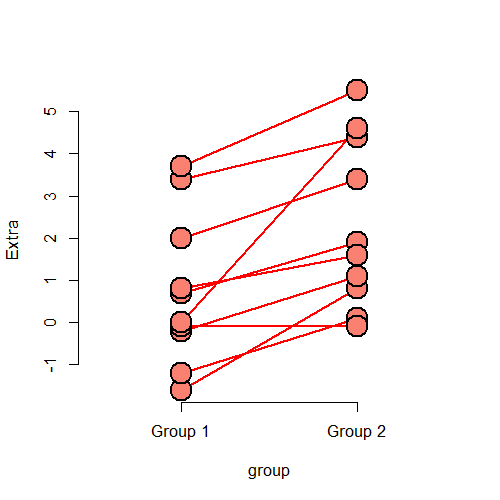
\includegraphics{sleep.png}
\caption{sleep}
\end{figure}

A lot of variance is explained by grouping the two groups. Pairing of
independent groups can hence really mess things up!.

\hypertarget{example-independent-groups-t-test.}{%
\section{Example: independent groups
t-test.}\label{example-independent-groups-t-test.}}

\begin{Shaded}
\begin{Highlighting}[]
\KeywordTok{library}\NormalTok{(datasets); }\KeywordTok{data}\NormalTok{(ChickWeight); }\KeywordTok{library}\NormalTok{(reshape2)}
\CommentTok{##define weight gain or loss}
\NormalTok{wideCW <-}\StringTok{ }\KeywordTok{dcast}\NormalTok{(ChickWeight, Diet }\OperatorTok{+}\StringTok{ }\NormalTok{Chick }\OperatorTok{~}\StringTok{ }\NormalTok{Time, }\DataTypeTok{value.var =} \StringTok{"weight"}\NormalTok{)}
\KeywordTok{names}\NormalTok{(wideCW)[}\OperatorTok{-}\NormalTok{(}\DecValTok{1} \OperatorTok{:}\StringTok{ }\DecValTok{2}\NormalTok{)] <-}\StringTok{ }\KeywordTok{paste}\NormalTok{(}\StringTok{"time"}\NormalTok{, }\KeywordTok{names}\NormalTok{(wideCW)[}\OperatorTok{-}\NormalTok{(}\DecValTok{1} \OperatorTok{:}\StringTok{ }\DecValTok{2}\NormalTok{)], }\DataTypeTok{sep =} \StringTok{""}\NormalTok{)}
\KeywordTok{library}\NormalTok{(dplyr)}
\NormalTok{wideCW <-}\StringTok{ }\KeywordTok{mutate}\NormalTok{(wideCW,}
  \DataTypeTok{gain =}\NormalTok{ time21 }\OperatorTok{-}\StringTok{ }\NormalTok{time0}
\NormalTok{)}
\end{Highlighting}
\end{Shaded}

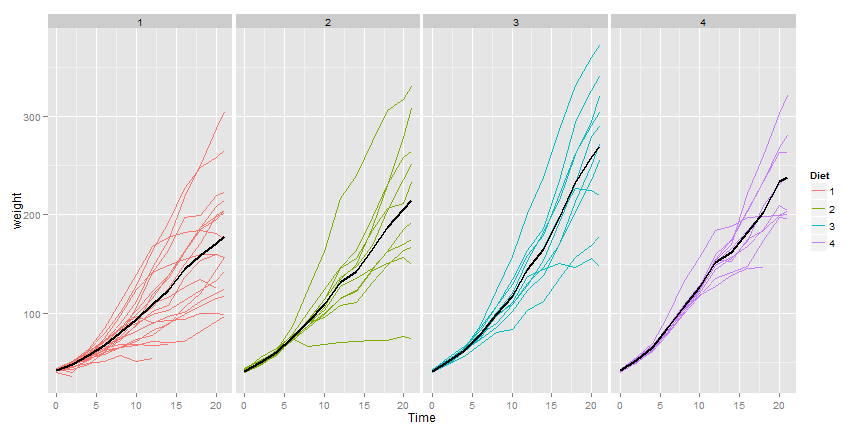
\includegraphics{chick1.png} 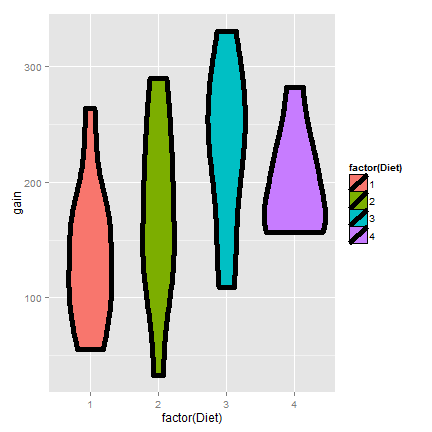
\includegraphics{chick2.png}

Now let's do a t interval comparing groups 1 and 4. We'll show the two
intervals, one assuming that the variances are equal and one assuming
otherwise.

\begin{Shaded}
\begin{Highlighting}[]
\NormalTok{wideCW14 <-}\StringTok{ }\KeywordTok{subset}\NormalTok{(wideCW, Diet }\OperatorTok\StringTok{ }\KeywordTok{c}\NormalTok{(}\DecValTok{1}\NormalTok{, }\DecValTok{4}\NormalTok{))}
\KeywordTok{rbind}\NormalTok{(}
  \KeywordTok{t.test}\NormalTok{(gain }\OperatorTok{~}\StringTok{ }\NormalTok{Diet, }\DataTypeTok{paired =} \OtherTok{FALSE}\NormalTok{, }\DataTypeTok{var.equal =} \OtherTok{TRUE}\NormalTok{, }\DataTypeTok{data =}\NormalTok{ wideCW14)}\OperatorTok{$}\NormalTok{conf,}
  \KeywordTok{t.test}\NormalTok{(gain }\OperatorTok{~}\StringTok{ }\NormalTok{Diet, }\DataTypeTok{paired =} \OtherTok{FALSE}\NormalTok{, }\DataTypeTok{var.equal =} \OtherTok{FALSE}\NormalTok{, }\DataTypeTok{data =}\NormalTok{ wideCW14)}\OperatorTok{$}\NormalTok{conf}
\NormalTok{)}
\end{Highlighting}
\end{Shaded}

\begin{verbatim}
##           [,1]      [,2]
## [1,] -108.1468 -14.81154
## [2,] -104.6590 -18.29932
\end{verbatim}

For the time being, let's interpret the equal variance interval. Since
the interval is entirely below zero it suggest that group 1 had less
weight gain than group 4 (at 95\% confidence).

\hypertarget{hypothesis-testing}{%
\section{Hypothesis testing:}\label{hypothesis-testing}}

Hypothesis testing is concerned with making decisions using data. *
Deciding between two hypotheses is a core activity in scientific
discovery. Statistical hypothesis testing is the formal inferential
framework around choosing between hypotheses.

\begin{itemize}
\item
  A null hypothesis is specified that represents the status quo, usually
  labeled \(H_0\)
\item
  The null hypothesis is assumed true and statistical evidence is
  required to reject it in favor of a research or alternative
  hypothesis.
\end{itemize}

\hypertarget{example}{%
\subsection{Example}\label{example}}

\begin{itemize}
\item
  A respiratory disturbance index of more than \(30\) events / hour,
  say, is

  considered evidence of severe sleep disordered breathing (SDB).
\item
  Suppose that in a sample of \(100\) overweight subjects with other

  risk factors for sleep disordered breathing at a sleep clinic, the

  mean RDI was \(32\) events / hour with a standard deviation of \(10\)
  events / hour.
\item
  We might want to test the hypothesis that

  \begin{itemize}
  \item
    \(H_0 : \mu = 30\)
  \item
    \(H_a : \mu > 30\)
  \item
    where \(\mu\) is the population mean RDI.
  \end{itemize}
\end{itemize}

\hypertarget{hypothesis-testing-1}{%
\subsection{Hypothesis testing}\label{hypothesis-testing-1}}

\begin{itemize}
\item
  The alternative hypotheses are typically of the form \(<\), \(>\) or
  \(\neq\)
\item
  Note that there are four possible outcomes of our statistical decision
  process
\end{itemize}

\begin{longtable}[]{@{}lll@{}}
\toprule
Truth & Decide & Result\tabularnewline
\midrule
\endhead
\(H_0\) & \(H_0\) & Correctly accept nul: True Positivel\tabularnewline
\(H_0\) & \(H_a\) & Type I error: False Positive\tabularnewline
\(H_a\) & \(H_a\) & Correctly reject null:True Negative\tabularnewline
\(H_a\) & \(H_0\) & Type II error: False Negative\tabularnewline
\bottomrule
\end{longtable}

A reasonable strategy would be to reject the null hypothesis
if\(\bar X\) was larger than some constant, say \(C\)

Typically, \(C\) is chosen so that the probability of a Type I error,
\(\alpha\), is \(.05\) (or some other relevant constant)

\(\alpha\) = Type I error rate = Probability of rejecting the null
hypothesis when, in fact, the null hypothesis is correct

\begin{itemize}
\item
  For \(\alpha=0.05\), 95th percentile of Normal Distribution is 1.645
  sd away from the mean.
\item
  We would just reject \(H_0\) because the Z-score:
  \[\frac{32 - 30}{10 / \sqrt{100}} = 2\] is greater than \(1.645\)
\item
  Or, whenever \(\sqrt{n} (\bar X - \mu_0) / s > Z_{1-\alpha}\)
\item
  The \(Z\) test for \(H_0:\mu = \mu_0\) versus

  \begin{itemize}
  \tightlist
  \item
    \(H_1: \mu < \mu_0\)
  \item
    \(H_2: \mu \neq \mu_0\)
  \item
    \(H_3: \mu > \mu_0\)
  \item
    Test statistic \[TS = \frac{\bar{X} - \mu_0}{S / \sqrt{n}}\]
  \end{itemize}
\end{itemize}

In General, Reject the null hypothesis when

\begin{itemize}
\tightlist
\item
  \(TS \leq -Z_{1 - \alpha}\)
\item
  \(|TS| \geq Z_{1 - \alpha / 2}\) (Two sided test)
\item
  \(TS \geq Z_{1 - \alpha}\)
\end{itemize}

\hypertarget{t-hypothesis-test}{%
\section{T Hypothesis Test:}\label{t-hypothesis-test}}

Consider our example again. Suppose that \(n= 16\) (rather than
\(100\)). Then consider that

\[.05 = P\left(\frac{\bar X - 30}{s / \sqrt{16}} \geq t_{1-\alpha, 15} ~|~ \mu = 30 \right)\]

\begin{itemize}
\tightlist
\item
  So that our test statistic is now \[\sqrt{16}(32 - 30) / 10 = 0.8 \],
  while the critical value is \[t_{1-\alpha, 15} = 1.75\]
\end{itemize}

-Since our Test Statitic,0.8 \textless{} 1.75, We now fail to reject.

\hypertarget{two-sided-tests}{%
\subsection{Two sided tests:}\label{two-sided-tests}}

\begin{itemize}
\item
  Suppose,Now that we would reject the null hypothesis if in fact the

  mean was too large or too small
\item
  That is, we want to test the alternative \(H_a : \mu \neq 30\)
\item
  Then note
\end{itemize}

\[ \alpha = P\left(\left. \left|\frac{\bar X - 30}{s /\sqrt{16}}\right| > t_{1-\alpha/2,15} ~\right|~ \mu = 30\right) \]

\begin{itemize}
\item
  That is we will reject if the test statistic, \(0.8\), is either

  too large or too small, but the critical value is calculated using

  \(\alpha / 2\)
\item
  In our example the critical value is \(2.13\), so we fail to reject
  since \(0.8 < 2.13\).
\end{itemize}

\hypertarget{t-test-in-r}{%
\subsection{T test in R:}\label{t-test-in-r}}

\begin{Shaded}
\begin{Highlighting}[]
\KeywordTok{library}\NormalTok{(UsingR); }\KeywordTok{data}\NormalTok{(father.son)}

\KeywordTok{t.test}\NormalTok{(father.son}\OperatorTok{$}\NormalTok{sheight }\OperatorTok{-}\StringTok{ }\NormalTok{father.son}\OperatorTok{$}\NormalTok{fheight)}
\end{Highlighting}
\end{Shaded}

\begin{verbatim}
## 
##  One Sample t-test
## 
## data:  father.son$sheight - father.son$fheight
## t = 11.789, df = 1077, p-value < 2.2e-16
## alternative hypothesis: true mean is not equal to 0
## 95 percent confidence interval:
##  0.8310296 1.1629160
## sample estimates:
## mean of x 
## 0.9969728
\end{verbatim}

Notice R gives us a P-value.P-values are a convenient way to communicate
the results of a hypothesis test. When communicating a P-value, the
reader can perform the test at whatever Type I error rate that they
would like. Just compare the P-value to the desired Type I error rate
and if the P-value is smaller, reject the null hypothesis.

\begin{itemize}
\tightlist
\item
  P values can be used against the type I error rate \(\alpha\) to
  reject or accept \(H_0\).
\item
  A p-value indicates the probability under the Null Hypothesis of
  obtaining evidence as extreme or more extreme as we did.So, a small p
  value would indicate that either we observed a rare event or our
  \(H_0\) is incorrect.
\item
  Therefore, If \[p < \alpha \], we reject the null hypothesis, else we
  fail to reject.
\end{itemize}

\hypertarget{p-value-example-1-binomial}{%
\subsection{P-value example 1:
(Binomial)}\label{p-value-example-1-binomial}}

Suppose, a friend has 8 children, 7 of which are girls and none are
twins. If each gender has an independent probability of 50\% of each
birth, what's the probabilty of getting 7 or more girls out of 8 births?
Let our Null Hypothesis \(H_0\) be that both genders have equal
probability of birth. And \(H_a\) be that probability of a girl birth is
more that probability of a boy birth. Then,

\begin{Shaded}
\begin{Highlighting}[]
\KeywordTok{pbinom}\NormalTok{(}\DecValTok{6}\NormalTok{,}\DataTypeTok{size=}\DecValTok{8}\NormalTok{,}\DataTypeTok{prob=}\FloatTok{0.5}\NormalTok{,}\DataTypeTok{lower.tail=}\NormalTok{F)}
\end{Highlighting}
\end{Shaded}

\begin{verbatim}
## [1] 0.03515625
\end{verbatim}

So, around 3.5\% chance of 7 or more girls out of 8. If we set our alpha
level to be 0.05. 0.035 \textless{} 0.05. Hence we reject \(H_0\).
Therefore, P(girl birth) \textgreater{} P(boy birth).

\hypertarget{p-value-example-2-poisson}{%
\subsection{P-value example 2:
(Poisson)}\label{p-value-example-2-poisson}}

Suppose that a hospital has an infection rate of 10 infections per 100
person/days at risk (rate=0.1). during the last month period. Assume
that an infection rate of 0.05 is an important benchmark.So if rate goes
above that they would implenent some quality control procedures. Should
the hospital get the expensive quality control procedures done? The key
question is: what's the probabilty of obtaining 10 or more infection per
100 person/days given rate of infection 0.05? Under: \(H_0\) :
\(\lambda=0.5\) so that \(\lambda*100\)=5. Consider \(H_a\):
\(\lambda>0.05\)

\begin{Shaded}
\begin{Highlighting}[]
\KeywordTok{ppois}\NormalTok{(}\DecValTok{9}\NormalTok{,}\FloatTok{0.05}\OperatorTok{*}\DecValTok{100}\NormalTok{,}\DataTypeTok{lower.tail =}\NormalTok{ F)}
\end{Highlighting}
\end{Shaded}

\begin{verbatim}
## [1] 0.03182806
\end{verbatim}

p-value : 0.03183. i.e.~3\% \[p=0.031<0.05\] * Therefore it's unlikely
for us to have seen as many as 10 infects per 100 person/day at risk if
the real infection rate was 5 infections per 100 person/day. So the
hospital probably should get the quality control procedures done.


\end{document}
